\makeatletter
\def\input@path{{../../}}
\makeatother
\documentclass[../../main.tex]{subfiles}

\graphicspath{
	{../../img/}
	{../img/}
	{img/}
}

\begin{document}

\section{Основная теорема о вычетах}

	Пусть $f(z)$ --- аналитическая в некоторой окрестности точки $z_0,$ которая является либо устранимой особой точкой,
	либо полюсом, либо существенно особой точкой, и во всех случаях изолированна, то есть в соответствующей ее окрестности нет других особых точек. Тогда в $0 < |z-z_0| < R \ f(z)$ можно разложить в соответствующий ряд Лорана:
	\[
		f(z) = \sum_{-\infty}^{+\infty}c_n(z-z_0)^n.
	\]
	
	Коэффициент $c_{-1}$ в этом разложении называется вычетом $f(z)$ в точке $z_0$ и обозначается 
	$c_{-1} = \underset{z_0}{res} f(z).$
	
	Используя формулу для коэффициентов Лорана, имеем:
	\[
		\begin{cases}
		c_n = \frac{1}{2\pi i} \ointctrclockwise\limits_{l} \frac{f(z)}{(z - z_0)^{n+1}}dz,\\
		n \in \Z.
		\end{cases}
	\]
	\begin{equation} \label{35.1}
		n = -1 \implies c_{-1} = \frac{1}{2\pi i} \ointctrclockwise\limits_{l} f(z)dz \implies 
		\ointctrclockwise\limits_{l} f(z)dz = 2\pi i c_{-1} = 2 \pi i \underset{z_0}{res} f(z).
	\end{equation}
	\eqref{35.1} позволяет вычислить интеграл ФКП в случае, когда известен соответствующий вычет. Из \eqref{35.1} следует, что есил $z_0$ --- правильная точка(либо точка аналитичности, либо устранимая особая точка), то 
	\[
		\underset{z_0}{res}f(z) = 0 \implies 
		\ointctrclockwise\limits_{l} f(z)dz = 0.
	\]
	
	\begin{thm}[Основная теорема о вычетах]
		Пусть $D$ --- односвязная ограниченная область и $f(z)$ --- аналитична в $D \setminus\{z_1, z_2, \ldots z_m\}.$
		Если  $f(z)$ --- непрерывна в $\overline{D}\setminus\{z_1, z_2, \ldots z_m\},$ 
		то тогда для любого замкнутого контура $l$ имеем
		\begin{equation} \label{35.2}
			I = \ointctrclockwise\limits_{l} f(z)dz = 2\pi i c_{-1} = 2 \pi i \sum_{k=1}^{m}\underset{z_k}{res} f(z).
		\end{equation}
	\end{thm}	
	\begin{proof}
		Воспользуемся методом отделения особенностей для многосвязных областей.
		
		Обычным образом показывается, что $I = \ointctrclockwise\limits_{l} f(z)dz,$ также как и при доказательстве теоремы Коши. 
		В силу \eqref{35.1} имеем $\ointctrclockwise\limits_{l} f(z)dz = 2\pi i c_{-1} = 2 \pi i \sum_{k=1}^{m}\underset{z_k}{res} f(z) \implies \eqref{35.2}.$
	\end{proof}	

	\rems
	\begin{enumerate}
		\item Если $D$ --- многосвязная, то имеет место \eqref{35.2}, только берется полная граница $D.$
		\item Практическая польза \eqref{35.2}в том, что чтобы ее использовать, нужно знать вычеты (уметь их вычислять).
	\end{enumerate}
	
	\section{Вычисление вычетов относительно полюса}
	Пусть $z_0$ --- простой полюс для $f(z),$ тогда в соответствующей выколотой окрестности $z_0$
	\[
		f(z) = \frac{c_{-1}}{z-z_0} + c_0 + c_1(z-z_0) + \ldots,
	\]
	\[
		\begin{cases}
		f(z) \sim \frac{c_{-1}}{z - z_0},\\
		z \to z_0.
		\end{cases}
	\]
	\[
		(z-z_0)f(z) = c_{-1} + c_0(z-z_0) + c_1(z-z_0)^2 + \ldots \underset{z \to z_0}{\to} c_{-1}. 	
	\]
	\begin{equation} \label{35.3}
		\underset{z_0}{res} f(z) = c_1 = \lim\limits_{z\to z_0}(z-z_0)f(z).
	\end{equation}
	
	
	Отметим, что \eqref{35.3} принимает наиболее простой вид в случае, когда $f(z) = \frac{\varphi(z)}{\psi(z)},$ где 
	$\varphi(z)$ --- аналитическая в точке $z_0, \psi(z)$ такова, что $z_0$ --- простой нуль $(\psi(z_0) = 0, \psi'(z_0) \ne 0).$
	\[
		\underset{z_0}{res} f(z) = \lim\limits_{z\to z_0}\frac{(z-z_0)\varphi(z)}{\psi(z) - \psi(z_0)} = 
		\lim\limits_{z\to z_0}\frac{\varphi(z)}{\frac{\psi(z) - \psi(z_0)}{z - z_0}} = \frac{\varphi(z_0)}{\psi'(z_0)}.
	\]
	\begin{equation}\label{35.4}
		\underset{z_0}{res} \frac{\varphi(z)}{\psi(z)} = \frac{\varphi(z_0)}{\psi'(z_0)}.
	\end{equation}
	
	В случае рациональной функции: $f(z) = \frac{P(z)}{Q(z)}$ --- правильная дробь $(\deg P < \deg Q),$ в случае когда у знаменателя все корни $z_1, z_2, \ldots, z_m$ простые (кратности 1), имеем разложение на простые дроби 
	\[
		f(z) = \sum_{k=1}^{m}\frac{A_n}{z-z_k},
	\]  
	\[
		\begin{cases}
		A_k = 	\underset{z_0}{res} \frac{P(z)}{Q'(z)}, \\
		k = \overline{1, m}.
		\end{cases}
	\]
	\textbf{Случай порядка $p \in \N:$}
	
	Имеем разложение 
	\[
		f(z) = \frac{c{-p}}{(z-z_0)^{p}} + \frac{c{-p+1}}{(z-z_0)^{p-1}} + \ldots + 
		\frac{c_{-1}}{z-z_0} + c_0 + c_1(z-z_0) + \ldots,
	\]
	\[
		(z-z_0)^pf(z) = c_{-p} + c_{-p+1}(z-z_0) + \ldots + c_{-1}(z-z_0)^{p-1} + c_0(z-z_0)^p.
	\]
	
	Дифференцируя это равенство $p-1$ раз, получим:
	\[
		((z-z_0)^pf(z))^{(p-1)} = (p-1)!c_{-1} + 2 \cdot 3 \cdot \ldots \cdot (p-1)c_0(z-z_0) + \ldots 
		\underset{z \to z_0}{\to} (p-1)!c_{-1}
	\]
	\begin{equation} \label{35.5}
		\underset{z_0}{res} f(z) = c_{-1} = \frac{1}{(p-1)!}
		\lim\limits_{z\to z_0} ((z-z_0)^pf(z))^{(p-1)}
	\end{equation}
	Отметим, что \eqref{35.5} применима не только, когда известно, что $z_0$ --- полюс порядка $p,$ но и когда известно, что $x_0$ --- полюс порядка не выше $p.$
	
	Наиболее простой вид у \eqref{35.5} получается в случае, если $\begin{cases}
	f(z)  = \frac{\varphi(z)}{(z-z_0)^p}, \\
	f(z) \text{ --- аналитическая.}
	\end{cases}$
	\begin{equation} \label{35.6}
		\underset{z_0}{res}  \frac{\varphi(z)}{(z-z_0)^p} = \frac{1}{(p-1)!}
		 \lim\limits_{z\to z_0} \left((z-z_0)^p \frac{\varphi(z)}{(z-z_0)^p}\right)^{(p-1)} = 
		 \frac{1}{(p-1)!} \varphi^{(p-1)}(z)\bigg|_{z = z_0} = \frac{\varphi^{(p-1)}(z_0)}{(p-1)!}.
	\end{equation}
	Как и \eqref{35.5}, \eqref{35.6} справедлива в случае, когда $z_0$ полюс порядка не выше $p$.
	
	\textbf{Случай, когда $z_0$ --- существенно особая точка}
	
	В этом случае вычет для $f(z) $ находим либо в силу определения, либо через сумму всех вычетов, котрая по теореме о вычетах с учетом бесконечно удаленной точки равна нулю.
	
\section{Ряд Лорана и вычеты БУТ(бесконечно удаленной точки)}

	Если $z_0$ --- конечная особая точка, то в соответствующей окрестности имеем разложение в ряд Лорана:
	
	\[
	f(z) = \sum_{n=-\infty}^{+\infty}c_n(z-z_0)^n=\dots+
	\frac{c_{-2}}{(z-z_0)^2}+\frac{c_{-1}}{(z-z_0)}+c_0+c_1(z-z_0)+\dots .
	\] 
	
	В частности, $z_0=0, 0< \mid z\mid < R:
	 f(z)=\sum\limits_{n=-\infty}^{+\infty} \frac{c_{-n}}{z^n}$.
	 
	$\sum\limits_{n=1}^{+\infty} \frac{c_{-n}}{z^n}$ --- главная часть,
	$\sum\limits_{n=0}^{+\infty} c_{n}z^n$ --- правильная часть. 
	 
	 Если $\mid z \mid > R$, а $f(z)$ --- аналитична, то полагаем: 
	 $t=\cfrac{1}{z} \implies \mid t \mid = \cfrac{1}{\mid z \mid} <
	 \cfrac1R=R_0$ и вводим
	 $\begin{cases}
	 g(t)=f\left(\cfrac 1t\right)\\
	 0<\mid t \mid < R 
	 \end{cases}.$
	 Имеем разложение 
	 \[g(t) = \sum\limits_{n=-\infty}^{+\infty}d_nt^n=
	 \dots + \cfrac{d_{-2}}{t^2} + \cfrac{d_{-1}}{t}+d_0+d_1t+\dots.
	 \]
	 
	 Для исходной функции: $f(z)=g\left(\cfrac1z\right)=\sum\limits_{n=-\infty}^{+\infty}
	 \frac{d_n}{z^n}=\dots + \cfrac{d_{2}}{t^2} + \cfrac{d_{1}}{t}
	 +d_0+d_{-1}t+d_{-2}z^2+\dots$, поэтому любое разложение в
	  окрестности нуля есть разложение в окрестности БУТ:
	 \[
	 f(z)=\underbrace{\dots+\frac{c_{-2}}{z^2}+\cfrac{c_{-1}}{z}+c_0}_{
	 \text{правильная часть }z=\infty}+
	 \underbrace{c_1z+\dots}_{\text{главная часть }z=\infty} .
	 \] 
	 
	 Тогда в зависимости от вида главной части для $z=\infty$ дают классификацию особенностей по аналогии с обычным случаем:
	 \begin{itemize}
	 	\item[а)] $z=\infty$ --- УОТ, когда главная часть отсутствует, т.~е.
	 	$\exists\lim\limits_{z\rightarrow \infty} f(z)=c_0\in \C$
	 	\item[б)] $z=\infty$ --- полюс, порядка $p\neq 0$, если в 
	 	главной части имеем только $p\neq 0$ слагаемых, то есть 
	 	$
	 	\begin{cases}
	 	f(z)=c_0+c_1z+\dots+c_pz^p+\sum\limits_{n=0}^{+\infty}\cfrac{c_n}
	 	z^n\\
	c_p\neq 0
	 	\end{cases}
	 	$ 
	 \item[в)] $z=\infty$ --- СОТ, если главная часть содержит бесконечное число ненулевых слагаемых. Для нахождения вычетов БУТ использвется тот факт, что сумма вычетов, в том числе и БУТ, равна нулю, а значит 
	 $\sum\limits_{k=1}^m\underset{z_k}{res}+\underset{\infty}{res}f(z)=0 \implies\underset{\infty}{res}f(z)-\sum\limits_{k=1}^m \underset{z_k}{res}f(z)$, либо используются формулы. аналогичные для конечных особенностей. При этом, когда конечная особенность является УОТ, и вычет в ней равен нулю, имеем 	$\underset{\infty}{res}f(z)=-c_{-1}.$ Он не обязательно будет нулевым, даже если $z=\infty$ --- УОТ.
	 
	 \begin{itemize}
	 	\item[1)] В разложении $f(z)$ в окрестности $z=\infty$ нет главной части, и значит, это УОТ, и тогда $f(z)=c_0+\cfrac{c_{-1}}{z}+\cfrac{c_{-2}}{z^2}+ \dots$ . В этом случае 
	 	$c_0=\lim\limits_{z\rightarrow \infty}f(z)=f(\infty)\in \R$, тогда 
	 	$(f(z)-f(\infty))z=c_{-1}+\cfrac{c_{-2}}{2}+ \dots\underset{z\rightarrow\infty}{\rightarrow}c_{-1}$. В этом случае имеем 	
	 	
	 	\begin{equation}\label{35.7}
	 	\underset{\infty}{res}f(z)=-c_{-1}=\lim\limits_{z-\rightarrow\infty}z(f(\infty)-f(z)).
	 	\end{equation}
	 	
	 	Из \ref{35.7} следует, что если $z=\infty$ --- нуль кратности $m$, то $f(z)=\cfrac{c_{-m}}{z^m}+ \cfrac{c_{-m+1}}{z^{m-1}}+\dots\sim \cfrac{c_{-1}}{z}, c_m\neq0$.
	 
	 	\[
	 	\underset{\infty}{res}f(z)=
	 	\begin{cases}
	 		-c_{-1}, m=1,\\
	 		0, m>1.
	 	\end{cases}
	 	\]
	 	
	 	\item[2)]
	 	$z=\infty$ --- полюс порядка $p$.
	 	
	 	\[
	 	\begin{cases}
	 	f(z)=\dots+\cfrac{c_{-2}}{z^2}+\cfrac{c_{-1}}{z}+c_0+c_1z+c_pz^p,\\
	 	c_p\neq0.
	 	\end{cases}
	 	\]
	 	
	 	Дифференцируя обе части $(p+1)$ раз, получим:
	 	
	 	\[
	 	f^{(p+1)}(z)=\dots+\cfrac{(-1)^{p}c_{-2}\cdot2\cdot3\cdot\dots \cdot(p+2)}{z^{p+3}}+\cfrac{(-1)^{p+1}c_{-1}(p+1)!}{z^{p+2}}+0\implies
	 	z^{p+2}f^{(p+1)}(z)=\dots+\cfrac{const}{z}+(-1)^{p+1}c_{-1}(p+1)! \underset{z\rightarrow \infty}{\rightarrow}(-1)^{p+1}c_{-1}(p+1)!.
	 	\]
	 	
	 	\begin{equation}
	 	\underset{\infty}{res}f(z)=-c_{-1}=\cfrac{(-1)^p}{(p+1)!} \lim\limits_{z\rightarrow\infty}z^{p+2}f^{(p+1)}(z).
	 	\end{equation}
	 	
	 	\item[3)] 
	 	БУТ является СОТ. В этом случае как правило считается через ряд Лорана. Отметим, что при применении вычетов на бесконечности при вычислении интегралов можно использовать особые точки как внутри области интегрирования, так и снаружи, с учетом БУТ, в силу того что сумма всех вычетов равна нулю:
	 	\[
	 	I=\oint\limits_lf(z)dz=2\pi i \sum_{i=1}^{k}\underset{z_j}{res}f(z)=-2\pi i\left(\sum_{j=k+1}^{m}\underset{z_j}{res}f(z)+\underset{\infty}{res}f(z)
	 	\right)=-\oint\limits_lf(z)dz.
	 	\]
	 	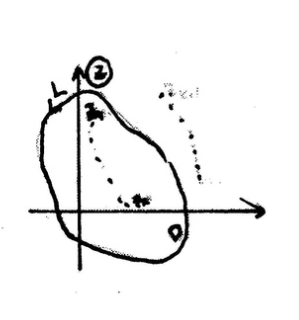
\includegraphics{lec_27}
	 \end{itemize}
	 \end{itemize}
\end{document}

